% THIS DOCUMENT IS TAILORED TO REQUIREMENTS FOR SCIENTIFIC COMPUTING.  IT SHOULDN'T
% BE USED FOR NON-SCIENTIFIC COMPUTING PROJECTS
\documentclass[12pt]{article}

\usepackage{amsmath, mathtools}
\usepackage{amsfonts}
\usepackage{amssymb}
\usepackage{graphicx}
\usepackage{colortbl}
\usepackage{xr}
\usepackage{hyperref}
\usepackage{longtable}
\usepackage{xfrac}
\usepackage{tabularx}
\usepackage{float}
\usepackage{siunitx}
\usepackage{booktabs}
\usepackage{caption}
\usepackage{pdflscape}
\usepackage{afterpage}

\usepackage[round]{natbib}

%\usepackage{refcheck}

\hypersetup{
    bookmarks=true,         % show bookmarks bar?
      colorlinks=true,       % false: boxed links; true: colored links
    linkcolor=red,          % color of internal links (change box color with linkbordercolor)
    citecolor=green,        % color of links to bibliography
    filecolor=magenta,      % color of file links
    urlcolor=cyan           % color of external links
}

%% Comments

\usepackage{color}

\newif\ifcomments\commentstrue %displays comments
%\newif\ifcomments\commentsfalse %so that comments do not display

\ifcomments
\newcommand{\authornote}[3]{\textcolor{#1}{[#3 ---#2]}}
\newcommand{\todo}[1]{\textcolor{red}{[TODO: #1]}}
\else
\newcommand{\authornote}[3]{}
\newcommand{\todo}[1]{}
\fi

\newcommand{\wss}[1]{\authornote{blue}{SS}{#1}} 
\newcommand{\plt}[1]{\authornote{magenta}{TPLT}{#1}} %For explanation of the template
\newcommand{\an}[1]{\authornote{cyan}{Author}{#1}}

%% Common Parts

\newcommand{\progname}{ProgName} % PUT YOUR PROGRAM NAME HERE
\newcommand{\authname}{Team \#, Team Name
\\ Student 1 name
\\ Student 2 name
\\ Student 3 name
\\ Student 4 name} % AUTHOR NAMES                  

\usepackage{hyperref}
    \hypersetup{colorlinks=true, linkcolor=blue, citecolor=blue, filecolor=blue,
                urlcolor=blue, unicode=false}
    \urlstyle{same}
                                


% For easy change of table widths
\newcommand{\colZwidth}{1.0\textwidth}
\newcommand{\colAwidth}{0.13\textwidth}
\newcommand{\colBwidth}{0.82\textwidth}
\newcommand{\colCwidth}{0.1\textwidth}
\newcommand{\colDwidth}{0.05\textwidth}
\newcommand{\colEwidth}{0.8\textwidth}
\newcommand{\colFwidth}{0.17\textwidth}
\newcommand{\colGwidth}{0.5\textwidth}
\newcommand{\colHwidth}{0.28\textwidth}

% Used so that cross-references have a meaningful prefix
\newcounter{defnum} %Definition Number
\newcommand{\dthedefnum}{GD\thedefnum}
\newcommand{\dref}[1]{GD\ref{#1}}
\newcounter{datadefnum} %Datadefinition Number
\newcommand{\ddthedatadefnum}{DD\thedatadefnum}
\newcommand{\ddref}[1]{DD\ref{#1}}
\newcounter{theorynum} %Theory Number
\newcommand{\tthetheorynum}{TM\thetheorynum}
\newcommand{\tref}[1]{TM\ref{#1}}
\newcounter{tablenum} %Table Number
\newcommand{\tbthetablenum}{TB\thetablenum}
\newcommand{\tbref}[1]{TB\ref{#1}}
\newcounter{assumpnum} %Assumption Number
\newcommand{\atheassumpnum}{A\theassumpnum}
\newcommand{\aref}[1]{A\ref{#1}}
\newcounter{goalnum} %Goal Number
\newcommand{\gthegoalnum}{GS\thegoalnum}
\newcommand{\gsref}[1]{GS\ref{#1}}
\newcounter{instnum} %Instance Number
\newcommand{\itheinstnum}{IM\theinstnum}
\newcommand{\iref}[1]{IM\ref{#1}}
\newcounter{reqnum} %Requirement Number
\newcommand{\rthereqnum}{R\thereqnum}
\newcommand{\rref}[1]{R\ref{#1}}
\newcounter{nfrnum} %NFR Number
\newcommand{\rthenfrnum}{NFR\thenfrnum}
\newcommand{\nfrref}[1]{NFR\ref{#1}}
\newcounter{lcnum} %Likely change number
\newcommand{\lthelcnum}{LC\thelcnum}
\newcommand{\lcref}[1]{LC\ref{#1}}

\usepackage{fullpage}

\newcommand{\deftheory}[9][Not Applicable]
{
\newpage
\noindent \rule{\textwidth}{0.5mm}

\paragraph{RefName: } \textbf{#2} \phantomsection 
\label{#2}

\paragraph{Label:} #3

\noindent \rule{\textwidth}{0.5mm}

\paragraph{Equation:}

#4

\paragraph{Description:}

#5

\paragraph{Notes:}

#6

\paragraph{Source:}

#7

\paragraph{Ref.\ By:}

#8

\paragraph{Preconditions for \hyperref[#2]{#2}:}
\label{#2_precond}

#9

\paragraph{Derivation for \hyperref[#2]{#2}:}
\label{#2_deriv}

#1

\noindent \rule{\textwidth}{0.5mm}

}

\begin{document}

\title{Centrality in Graphs} 
\author{Atiyeh Sayadi}
\date{\today}
	
\maketitle

~\newpage

\pagenumbering{roman}

\tableofcontents

~\newpage

\section*{Revision History}

\begin{tabularx}{\textwidth}{p{3cm}p{2cm}X}
\toprule {\bf Date} & {\bf Version} & {\bf Notes}\\
\midrule
January 29, 2024  & 1.0 & Initial drafts\\
Feburary 4, 2024  & 1.0 & The first review\\
Feburary 14, 2024  & 1.0 & The second review\\

\bottomrule
\end{tabularx}

~\\

~\newpage

\section{Reference Material}

This section records information for easy reference.

\subsection{Table of Units}

In this project there is no special unit. 

\subsection{Table of Symbols}

The table that follows summarizes the symbols used in this document along with
their units.  The choice of symbols was made to be consistent with the heat
transfer literature and with existing documentation for solar water heating
systems.  The symbols are listed in alphabetical order.

\renewcommand{\arraystretch}{1.2}
%\noindent \begin{tabularx}{1.0\textwidth}{l l X}
\noindent \begin{longtable*}{l l p{12cm}} \toprule
\textbf{symbol} & \textbf{unit} & \textbf{description}\\
\midrule 
CC($\mathit i$)& \si[per-mode=symbol] {-} & Closeness Centrality of node i
\\DC($\mathit i$) & \si[per-mode=symbol] {-} & Degree Centrality of node i
which heat is transferred in
\\ 
\bottomrule
\end{longtable*}
\

\subsection{Abbreviations and Acronyms}

\renewcommand{\arraystretch}{1.2}
\begin{tabular}{l l} 
  \toprule		
  \textbf{symbol} & \textbf{description}\\
  \midrule 
  A & Assumption\\
  DD & Data Definition\\
  GD & General Definition\\
  GS & Goal Statement\\
  IM & Instance Model\\
  LC & Likely Change\\
  PS & Physical System Description\\
  R & Requirement\\
  SRS & Software Requirements Specification\\
CIG &  Centrality in Graphs: finding the most importamt nodes\\
  TM & Theoretical Model\\
  \bottomrule
\end{tabular}\\

\

\subsection{Mathematical Notation}
 There is no mathematical notation.

\section{Introduction}


Analyzing networks using graph-related concepts has been one of the most interesting areas of study for professionals. Among these concepts, centrality and identifying the most effective members of the network are crucial for some studies. This project attempted to identify the most important nodes in a given graph, represented in the form of a matrix of nodes and relationships, using degree centrality and closeness centrality methods. In fact, the goal is to calculate the centrality measures of each node in the graph using both of the mentioned methods.

\subsection{Purpose of Document}
The aim of creating this document is to outline the needs, conditions, goals, and etc. that the project will be designed and developed based on. Moreover, it will help ensure a more purposeful testing and approval process in the future and after implementation.

\subsection{Scope of Requirements} 


This project does not encompass various methods for calculating centrality in graphs. In other words, it only utilizes the closeness  and degree methods. Additionally, selecting the best criterion for centrality computation is not within the scope of this project's implementation agenda. For instance, other central criteria such as flexibility, pressure, power, etc., will not be calculated by the software. Lastly, weighted and directed graphs will not be examined in this project.

\subsection{Characteristics of Intended Reader} \label{sec_IntendedReader}


Readers of this document need to have sufficient knowledge about graphs, their properties and types, and network analysis in order to have a better understanding of these texts. Additionally, a high level of computer expertise is not required to understand this document.

\subsection{Organization of Document}

This document follows the structure proposed by \citet{SmithandLai2005}, covering all opportunities, requirements, definitions, etc. So, readers can start by looking at the goal statements and then dive into the theoretical model to fully understand the system.

\section{General System Description}

This section provides general information about the system.  It identifies the
interfaces between the system and its environment, describes the user
characteristics and lists the system constraints. 

\subsection{System Context}


Looking at Figure 1 gives you a basic idea of the system. First, it reads a graph file with a graph. Then, it calculates closeness measures for each node using centrality and closeness definitions, giving two arrays as output for the given graph.

\begin{figure}[h!]
\begin{center}
 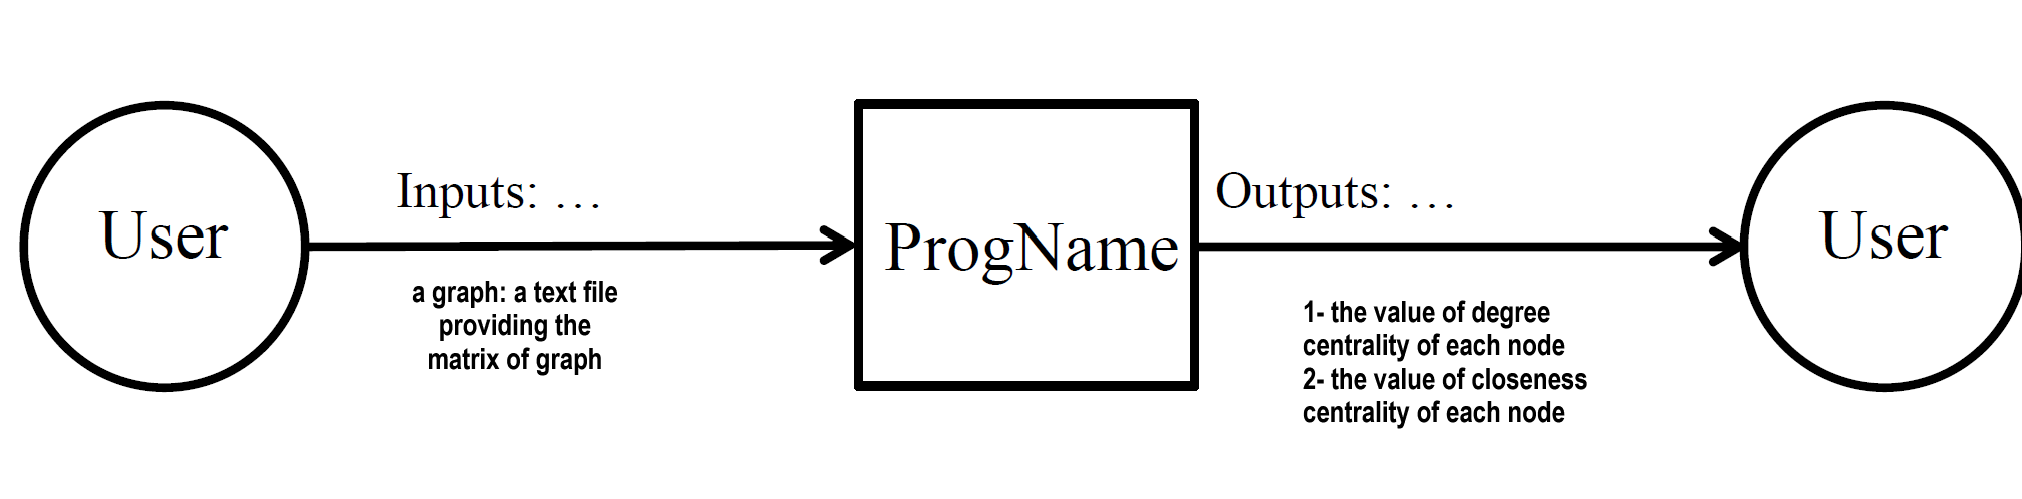
\includegraphics[width=0.6\textwidth]{srspicture}
\caption{System Context}
\label{Fig_SystemContext} 
\end{center}
\end{figure}


\begin{itemize}
\item User Responsibilities: 
\begin{itemize}
\item The matrix should be normalized.
\end{itemize}
\item \ CIG Responsibilities:
\begin{itemize}
\item Read the input file
\item Calculating degree and closeness centrality for each node in the graph correctly
\end{itemize}
\end{itemize}




\subsection{User Characteristics} \label{SecUserCharacteristics}
Users of this system should have sufficient familiarity with graphs and network analysis concepts to understand the program's output based on their input, which includes measures of centrality, degree, and proximity for each node. They should also be able to upload different files if needed. Since an interface is not designed for data entry, the user should be able to input the file directly into the program's source code.

\subsection{System Constraints}


This system does not examine weighted or directed graphs. Additionally, it does not encompass all types of centrality calculation methods.

\section{Specific System Description}

Consider having a graph representing a social network. We aim to identify the most central individuals in this network using the concept of centrality. Firstly, the social network needs to be introduced to the system in the form of a graph. In fact, it means that the network graph will be introduced to the system as an input in the form of a matrix. Then, the software calculates the centrality measures, specifically degree centrality and closeness centrality, for each node individually and ultimately computes them for all members of the network.

\subsection{Problem Description} \label{Sec_pd}

We have a graph representing a social network, and we aim to identify the most central individuals in this network using the concept of centrality. In other words, finding the most important members in a network in terms of their connections with other members is the main objective of this project.

\subsubsection{Terminology and  Definitions}

\begin{itemize}
\item \textbf{Graph:}  A collection of nodes connected by edges.

\item \textbf{Node:} Members in graphs.
\item \textbf{Edge:} Connections between nodes in graphs.

\item \textbf{Centrality:} Measure used to identify the most important nodes in a network.
\item \textbf{Degree:}  Number of direct connection that each node has.


\end{itemize}

\subsubsection{Physical System Description} \label{sec_phySystDescrip}

This project can model any network in which directionality is not significant, in the form of an undirected graph. In this network, it is preferred that there are no isolated nodes, although their presence does not disrupt computations, it increases the complexity of analysis. In fact, all networks with bidirectional communication paths can be modeled by this system.


\subsubsection{Goal Statements}


\begin{itemize}

\item[GS\refstepcounter{goalnum}\thegoalnum \label{g_degree}:] 
Calculating degree centrality for each node.
\item[GS\refstepcounter{goalnum}\thegoalnum \label{g_closeness}:]
Calculating closeness centrality for each node.

\end{itemize}

\subsection{Solution Characteristics Specification}

As previously mentioned, the solution presented in this system is only applicable to networks where the direction of communication between members is not significant, in other words, bidirectional relationships. Additionally, networks where communications do not have varying weights or values can be read as input in this system.

\subsubsection{Assumptions} \label{sec_assumpt}

To simplify the calculations, some assumptions have been made in this software:

\begin{itemize}

\item[A\refstepcounter{assumpnum}\theassumpnum \label{A_directed}:]
The graph is undirected.

\item[A\refstepcounter{assumpnum}\theassumpnum \label{A_weighted}:]
The length of each edge is equal to 1.
\end{itemize}

\subsubsection{Theoretical Models}\label{sec_theoretical}


The purpose of this project is to calculate centrality and proximity measures in a graph. Therefore, it is necessary to become more familiar with this concept accurately.

~\newline

\noindent
\deftheory
% #2 refname of theory
{TM:DC}
% #3 label
{Degree Centrality}
% #4 equation
{${DC (i)= \frac{\sum \text{edge}(i,j)}{N - 1}}$ 
}
% #5 description
{
  Degree centrality looks at
how many connections each node has, and if a node has a lot of connections, it’s
considered more important.to calcute DC for each node we need at first calculate degree of node. Degree of node is the number of edged that are direcly connectod to the node. After that we should devide the result to the number of nodes in the graph -1.
}
% #6 Notes
{
None.
}
% #7 Source
{
  \url{https://www.geeksforgeeks.org/degree-centrality-centrality-measure/}
}
% #8 Referenced by
{
\dref{g_dc},\iref{i_dc}
}
% #9 Preconditions
{
None
}
% #1 derivation - not applicable by default
{}


\noindent
\deftheory
% #2 refname of theory
{TM:CC}
% #3 label
{Closeness Centrality}
% #4 equation
{ ${CC (i)= \frac{N-1}{\sum{d}(i,j)}}$ 
~\newline
 $d(i,j)  $= The shortest path from i to j.\\
}
% #5 description
{
It checks how close a node is to all the other nodes in the graph. To calculate average distance from node i to all other node, the sum of shortest path from node i to all other nodes should be computed, and the result must divide to total number of nodes -1. Then it must be reversed to find the CC node i.
}
% #6 Notes
{
None.
}
% #7 Source
{
  \url{https://en.wikipedia.org/w/index.php?title=Centrality&oldid=1176179277}
}
% #8 Referenced by
{
\dref{g_cc},\iref{i_cc}
}
% #9 Preconditions
{
None
}
% #1 derivation - not applicable by default
{}
~\newline

\subsubsection{General Definitions}\label{sec_gendef}

In this section you can finde some general about graph, centrality, degree centrality and closeness centrality.

~\newline


\noindent
\begin{minipage}{\textwidth}
\renewcommand*{\arraystretch}{1.5}
\begin{tabular}{| p{\colAwidth} | p{\colBwidth}|}
\hline
\rowcolor[gray]{0.9}
Number& GD\refstepcounter{defnum}\thedefnum\label{g_graph}\\
\hline
Label &\bf Graph \\
\hline
% Units&$MLt^{-3}T^0$\\
% \hline
SI Units&\si-\\
\hline
Equisions&\si-  \\
\hline
Description &
Graph is a collection of nodes connected by edges.
It has applications in many fields such as algorithm design and 
   analysis, game theory and network theory.

\\
\hline
  Source & https://www.geeksforgeeks.org/graph-types-and-applications/ \\
  \hline
  Ref.\ By & TM1, TM2,\dref{g_centrality},\dref{g_dc},\dref{g_cc},\ddref{degree},\iref{i_dc},\iref{i_cc}\\
  \hline
\end{tabular}
\end{minipage}\\
\noindent
\begin{minipage}{\textwidth}
\renewcommand*{\arraystretch}{1.5}
\begin{tabular}{| p{\colAwidth} | p{\colBwidth}|}
\hline
\rowcolor[gray]{0.9}
Number& GD\refstepcounter{defnum}\thedefnum\label{g_centrality}\\
\hline
Label &\bf Centrality \\
\hline
% Units&$MLt^{-3}T^0$\\
% \hline
SI Units&\si-\\
\hline
Equisions&\si-  \\
\hline
Description &
"Centrality" is a measure used to identify the most important nodes in a network.

\\

\hline
  Source & https://visiblenetworklabs.com/2021/04/16/understanding-network-centrality/ \\
  \hline
  Ref.\ By & TM1, TM2,\dref{g_dc},\dref{g_cc},\iref{i_dc},\iref{i_cc}\\
  \hline
\end{tabular}
\end{minipage}\\
\noindent
\begin{minipage}{\textwidth}
\renewcommand*{\arraystretch}{1.5}
\begin{tabular}{| p{\colAwidth} | p{\colBwidth}|}
\hline
\rowcolor[gray]{0.9}
Number& GD\refstepcounter{defnum}\thedefnum\label{g_dc}\\
\hline
Label &\bf Degree Centrality \\
\hline
% Units&$MLt^{-3}T^0$\\
% \hline
SI Units&\si-\\
\hline
Equisions&\  ${DC (i)= \frac{\sum \text{edge}(i,j)}{N - 1}}$ \\
\hline
Description &
Degree centrality looks at how many connections each node has, and if a node has a lot of connections, it’s considered more important.


\\

\hline
  Source & https://www.geeksforgeeks.org/degree-centrality-centrality-measure/ \\
  \hline
  Ref.\ By & TM1, \iref{i_dc}\\
  \hline
\end{tabular}
\end{minipage}\\


\noindent
\begin{minipage}{\textwidth}
\renewcommand*{\arraystretch}{1.5}
\begin{tabular}{| p{\colAwidth} | p{\colBwidth}|}
\hline
\rowcolor[gray]{0.9}
Number& GD\refstepcounter{defnum}\thedefnum\label{g_cc}\\
\hline
Label &\bf Centrality Centrality \\
\hline
% Units&$MLt^{-3}T^0$\\
% \hline
SI Units&\si-\\
\hline
Equisions&\  ${CC (i)= \frac{N-1}{\sum d(i,j)}}$ 
~\newline
$d(i,j)  $ = The shortest path from i to j.\\
\hline
Description &
Checks how close a node is to all the other nodes in the graph.

\\

\\
\hline
  Source & https://en.wikipedia.org/wiki/Centrality\\
  \hline
  Ref.\ By & TM2, \iref{i_cc}\\
  \hline
\end{tabular}
\end{minipage}\\


\subsubsection{Data Definitions}\label{sec_datadef}


In this section, a general definition of the degree of node, which is highly important in graph theory, is presented.

~\newline

\noindent
\begin{minipage}{\textwidth}
\renewcommand*{\arraystretch}{1.5}
\begin{tabular}{| p{\colAwidth} | p{\colBwidth}|}
\hline
\rowcolor[gray]{0.9}
Number& DD\refstepcounter{datadefnum}\thedatadefnum \label{degree}\\
\hline
Label& \bf The Degree of Node\\
\hline
Symbol &$-$\\
\hline
% Units& $Mt^{-3}$\\
% \hline
  SI Units & \-\\
  \hline
Equation& $Degree(i)=\sum edge(i,j)$ \\
  \hline
  Description & 
               
In graph theory, the degree of a node is the number of edges directly connected to it.
  \\
  \hline
 Sources& https://www.geeksforgeeks.org/degree-centrality-centrality-measure/ \\
  \hline
  Ref.\ By & TM1,\dref{g_graph},\dref{g_centrality},\dref{g_dc},\ddref{degree},\iref{i_dc}\\
  \hline
\end{tabular}
\end{minipage}\\
\noindent
\begin{minipage}{\textwidth}
\renewcommand*{\arraystretch}{1.5}
\begin{tabular}{| p{\colAwidth} | p{\colBwidth}|}
\hline
\rowcolor[gray]{0.9}
Number& DD\refstepcounter{datadefnum}\thedatadefnum \label{matrix}\\
\hline
Label& \bf The adjacency matrix\\
\hline
Symbol &$-$\\
\hline
% Units& $Mt^{-3}$\\
% \hline
  SI Units & \-\\
  \hline
Equation& - \\
  \hline
  Description & 
               
The adjacency matrix, also called the connection matrix, is a matrix containing rows and columns which is used to represent a simple labelled graph, with 0 or 1 in the position of (V$i$ , V$j$) according to the condition whether V$i$ and V$j$ are adjacent or not.
  \\
  \hline
 Sources& https://byjus.com/maths/adjacency-matrix/ \\
  \hline
  Ref.\ By & TM1,\dref{g_graph},\dref{g_centrality},\dref{g_dc},\dref{g_cc},\ddref{degree},\iref{i_dc}, ,\iref{i_cc}\\
  \hline
\end{tabular}
\end{minipage}\\

\subsubsection{Data Types}\label{sec_datatypes}


In this project, the input is a matrix of natural numbers representing nodes and edges, and the output is a set of floating-point numbers indicating the centrality of each node in the graph.


\subsubsection{Instance Models} \label{sec_instance}    


In this section, a computational model of  degree and closeness centrality for each node of the given graph is presented.

~\newline

%Instance Model 1

\noindent
\begin{minipage}{\textwidth}
\renewcommand*{\arraystretch}{1.5}
\begin{tabular}{| p{\colAwidth} | p{\colBwidth}|}
  \hline
  \rowcolor[gray]{0.9}
  Number& IM\refstepcounter{instnum}\theinstnum \label{i_dc}\\
  \hline
  Label& Degree Centrality\\
  \hline
  Input& \ddref{matrix}\\
  \hline
  Output& The value of degree centrality for each node \\
  \hline
  Description& it shows how many direct connection have the  the nodes in the graph. 
  \\
  \hline
  Sources& \url{https://en.wikipedia.org/wiki/Degree_(graph_theory)}
 \\
  \hline
  Ref.\ By & -\\
  \hline
\end{tabular}
\end{minipage}\\

%~\newline


~\newline
%Instance Model 2

\noindent
\begin{minipage}{\textwidth}
\renewcommand*{\arraystretch}{1.5}
\begin{tabular}{| p{\colAwidth} | p{\colBwidth}|}
  \hline
  \rowcolor[gray]{0.9}
  Number& IM\refstepcounter{instnum}\theinstnum \label{i_cc}\\
  \hline
  Label& Closeness Centrality\\
  \hline
  Input& \ddref{matrix}\\
  \hline
  Output& The value of closeness centrality for each node \\
  \hline
  Description& it shows how close the nodes are to others. 
  \\
  \hline
  Sources& \url{https://en.wikipedia.org/wiki/Centrality)}
 \\
  \hline
  Ref.\ By & -\\
  \hline
\end{tabular}
\end{minipage}\\

%~\newline


\subsubsection{Input Data Constraints} \label{sec_DataConstraints}    


The input utilizes a text file to present the matrix of relationships in the graph. In this matrix, the elements are integers greater than zero.

\begin{table}[!h]
  \caption{Input Variables} \label{TblInputVar}
  \renewcommand{\arraystretch}{1.2}
\noindent \begin{longtable*}{l l l l c} 
  \toprule
  \textbf{Var} & \textbf{Physical Constraints} & \textbf{Software Constraints} &
                             \textbf{Typical Value} & \textbf{Uncertainty}\\
  \midrule 
  $Matrix  M$ & $|M| > 0$ & Integer value &  1  & \,
  \\
  \bottomrule
\end{longtable*}
\end{table}



\subsubsection{Properties of a Correct Solution} \label{sec_CorrectSolution}

\noindent
Output of this software is a set of numbers representing the centrality of each node in both methods. This value for each method ranges between zero and one.
\begin{table}[!h]
\caption{Output Variables} \label{TblOutputVar}
\renewcommand{\arraystretch}{1.2}
\noindent \begin{longtable*}{l l} 
  \toprule
  \textbf{Var} & \textbf{Physical Constraints} \\
  \midrule 
  $DC(i)$ & $ 0 \leq DC(i) \leq 1$
  \\
 $CC(i)$ & $ 0 \leq CD(i) \leq 1$
\\
  \bottomrule
\end{longtable*}
\end{table}


\section{Requirements}

This section delineates the requirements of this project across various sections.

\subsection{Functional Requirements}

\noindent \begin{itemize}

\item[R\refstepcounter{reqnum}\thereqnum \label{R_Inputs}:] Degree centrality for all nodes ranges between zero and one.
\item[R\refstepcounter{reqnum}\thereqnum \label{R_Calculate}:] Degree centrality has been calculated for all nodes.

\item[R\refstepcounter{reqnum}\thereqnum \label{R_VerifyOutput}:] Closeness centrality for all nodes ranges between zero and one.

\item[R\refstepcounter{reqnum}\thereqnum \label{R_Output}:] Closeness centrality has been calculated for all nodes.


\end{itemize}



\subsection{Nonfunctional Requirements}
In this section, non-functional requirements of the software are expressed in the form of various criteria.

\noindent \begin{itemize}

\item[NFR\refstepcounter{nfrnum}\thenfrnum \label{NFR_Accuracy}:]
  \textbf{Accuracy} \
This software should be developed in a way that ensures the reliability and accuracy of output generation performance.
\item[NFR\refstepcounter{nfrnum}\thenfrnum \label{NFR_Usability}:] \textbf{Usability}
Codes should be developed in a manner and within an environment that allows them to be usable across different operating systems and conditions. Additionally, it's necessary for the user to be able to work with them comfortably.
\item[NFR\refstepcounter{nfrnum}\thenfrnum \label{NFR_Maintainability}:]
  \textbf{Maintainability} 
Efforts should be made to minimize side effects between functions at minimum. Additionally, it is necessary for the names of functions, variables, and parameters to clearly reflect their functionality.

\item[NFR\refstepcounter{nfrnum}\thenfrnum \label{NFR_Portability}:]
  \textbf{Portability}
The software must be designed in such a way that it can be executed in different conditions and environments.


\end{itemize}

\subsection{Rationale}


In this project, efforts have been made to avoid using weighted and directed graphs because these graph models increase computational complexity. Additionally, since the degree centrality and closeness centrality calculations yield different results in directed graphs, the computation methods would also differ.

\section{Likely Changes}    

\noindent \begin{itemize}

\item[LC\refstepcounter{lcnum}\thelcnum\label{LC_meaningfulLabel}:] In this project, it is possible that the programming environment may change.

\item[LC\refstepcounter{lcnum}\thelcnum\label{LC_meaningfulLabel}:]  The method of defining the matrix in the input file may change from n*2 to n*n.
\item[LC\refstepcounter{lcnum}\thelcnum\label{LC_meaningfulLabel}:]  Computations may also be performed on directed graphs.

\end{itemize}

\section{Unlikely Changes}    

\noindent \begin{itemize}

\item[LC\refstepcounter{lcnum}\thelcnum\label{LC_meaningfulLabel}:] The input file is a text file.
\item[LC\refstepcounter{lcnum}\thelcnum\label{LC_meaningfulLabel}:] Only two centrality methods, degree centrality and closeness centrality, are used.

\end{itemize}

\section{Traceability Matrices and Graphs}

The purpose of the traceability matrices is to provide easy references on what
has to be additionally modified if a certain component is changed.  Every time a
component is changed, the items in the column of that component that are marked
with an ``X'' may have to be modified as well.  Table~\ref{Table:trace} shows the
dependencies of theoretical models, general definitions, data definitions, and
instance models with each other. Table~\ref{Table:R_trace} shows the
dependencies of instance models, requirements, and data constraints on each
other. Table~\ref{Table:A_trace} shows the dependencies of theoretical models,
general definitions, data definitions, instance models, and likely changes on
the assumptions.

\afterpage{
\begin{table}[h!]
\centering
\begin{tabular}{|c|c|c|c|c|c|c|c|c|c|c|c|c|c|c|c|c|c|c|c|}
\hline
	&\aref{A_directed}&\aref{A_weighted}\\
\hline
TM1     & X& \\ \hline
TM2     & X& X \\ \hline
\dref{g_graph}     & & \\ \hline
\dref{g_centrality}    & & \\ \hline
\dref{g_dc}      & X& \\ \hline
\dref{g_cc}    & X& X \\ \hline
\ddref{degree}   & X& \\ \hline
\iref{i_dc}    & X&\\ \hline
\iref{i_cc}    & X& X\\ \hline
\end{tabular}
\caption{Traceability Matrix Showing the Connections Between Assumptions and Other Items}
\label{Table:A_trace}
\end{table}
}

\begin{table}[h!]
\centering
\begin{tabular}{|c|c|c|c|c|c|c|c|c|c|c|c|c|c|c|c|c|c|c|c|c|c|c|c|}
\hline        
	& TM1&TM2&\dref{g_graph}&\dref{g_centrality}&\dref{g_dc}&\dref{g_cc}&\ddref{degree}&\iref{i_dc}&\iref{i_cc}\\
\hline
TM1& & & & &X& & &X& \\ \hline
TM2& & & & & &X& & &X\\ \hline
\dref{g_graph}&X&X&X&X&X&X&X&X&X\\ \hline
\dref{g_centrality}& & & & & &X&X&X&X\\ \hline
\dref{g_dc}& & & & & & & &X&\\ \hline
\dref{g_cc}& & & & & & & & &X\\ \hline
\ddref{degree}&X& & X&X&X& & &X& \\ \hline
\iref{i_dc}& & & & & & & & & \\ \hline
\iref{i_cc}& & & & & & & & & \\ \hline
\end{tabular}
\caption{Traceability Matrix Showing the Connections Between Items of Different Sections}
\label{Table:trace}
\end{table}

\begin{table}[h!]
\centering
\begin{tabular}{|c|c|c|c|c|c|c|c|}
\hline
	&\iref{i_dc}& \iref{i_cc}\\ \hline
\rref{R_Inputs}          &X& X\\ \hline
\rref{R_Calculate}         & X&X\\ \hline
\rref{R_VerifyOutput}         &X&X \\ \hline
\rref{R_Output}         &X& X\\ \hline
\end{tabular}
\caption{Traceability Matrix Showing the Connections Between Requirements and Instance Models}
\label{Table:R_trace}
\end{table}


% \begin{figure}[h!]
% 	\begin{center}
% 		%\rotatebox{-90}
% 		{
% 			\includegraphics[width=\textwidth]{ATrace.png}
% 		}
% 		\caption{\label{Fig_ATrace} Traceability Matrix Showing the Connections Between Items of Different Sections}
% 	\end{center}
% \end{figure}


% \begin{figure}[h!]
% 	\begin{center}
% 		%\rotatebox{-90}
% 		{
% 			\includegraphics[width=0.7\textwidth]{RTrace.png}
% 		}
% 		\caption{\label{Fig_RTrace} Traceability Matrix Showing the Connections Between Requirements, Instance Models, and Data Constraints}
% 	\end{center}
% \end{figure}

\section{Development Plan}


For software development, first, the input file needs to be standardized and read from the input. Then, two centrality algorithms, degree centrality and closeness centrality, are implemented, and efforts are made to display the output with relying on computations and definitions of other matrices.

\section{Values of Auxiliary Constants}


 \textbf{Input matrix:}: as an input we have a matrix[n:2]. It means it has several rows and just two columns.


\newpage

\bibliographystyle {plainnat}
\bibliography {../../refs/References}.\newline

Newman. (2013). Networks: An Introduction.\\\\
Wasserman, S. and Faust, K. (1994).
Social Network Analysis: Methods and Applications.\\\\
https://www.geeksforgeeks.org/degree-centrality-centrality-measure/\\\\
https://en.wikipedia.org/wiki/Centrality\\
https://visiblenetworklabs.com/2021/04/16/understanding-networkcentrality/\\\\
https://www.geeksforgeeks.org/graph-types-and-applications/\\\\

\newpage{}
\section*{Appendix --- Reflection}

The information in this section will be used to evaluate the team members on the
graduate attribute of Lifelong Learning.  Please answer the following questions:

\begin{enumerate}
  \item Which of the courses you have taken, or are currently taking, will help
  your team to be successful with your capstone project. 
  \item What knowledge and skills will the team collectively need to acquire to
  successfully complete this capstone project?  Examples of possible knowledge
  to acquire include domain specific knowledge from the domain of your
  application, or software engineering knowledge, mechatronics knowledge or
  computer science knowledge.  Skills may be related to technology, or writing,
  or presentation, or team management, etc.  You should look to identify at
  least one item for each team member.
  \item For each of the knowledge areas and skills identified in the previous
  question, what are at least two approaches to acquiring the knowledge or
  mastering the skill?  Of the identified approaches, which will each team
  member pursue, and why did they make this choice?
\end{enumerate}

\end{document}